\section{Expérience D4} \label{expD4}
  \subsection{Objectif}
    En partant de la seconde architecture de \cite{Cleeremans_2007}, 
    comprendre de quelles manières un réseau de neurone connexionniste peut, à partir de ses propres paris
    sur son résultat, améliorer son comportement.
  
  
  \subsection{Architecture}
    \paragraph{Description}
      Un premier réseau de perceptron multicouche apprend à discrétiser des chiffres représentés
      par 256 (16x16) neurones d'entrées. Il est composé d'une couche cachée de 100 neurones.
      
      Un second réseau de perceptron apprend par renforcement le taux d'apprentissage et le
      momentum idéale en fonction des représentations du premier réseau. Ces paramètres sont 
      encodé sur 3 neurones de façon binaire. Au final, le taux d'apprentissage est définit 
      sur [0.1 ; 0.35] et le momentum sur [0.2 ; 0.85].
      
      L'apprentissage du second réseau, n'affecte pas les poids entre la couche d'entrée et la 
      couche cachée du premier réseau.
    \paragraph{Schéma}
      \begin{center}
	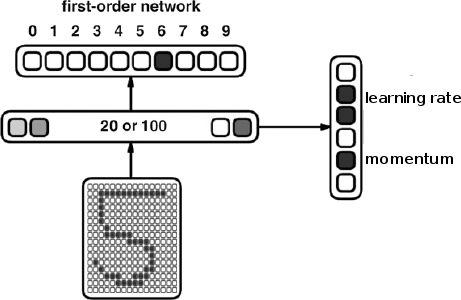
\includegraphics[width=220px]{data/expD4/schema.png}
      \end{center}
      
    \paragraph{Paramètres}
      \begin{center}
	\begin{tabular}{lr}
	  \begin{minipage}{230px}
	    \begin{itemize}
	      \item momentum : 0.9 sur les 2 réseaux
	      \item \textbf{1600 formes} de chiffres différents présentées (shuffle) \cite{Handwritten_256}
	      \item apprentissage 50 (formes) x 300 (époques)
	      
	    \end{itemize}
	  \end{minipage}
	  &
	  \begin{minipage}{230px}
	    \begin{itemize}
	      \item poids initialisés sur [-0.25 ; 0.25]
	      \item entrées valent 0 ou 1
	      \item sigmoïde à température 1
	      \item utilisation de biais
	    \end{itemize}
	  \end{minipage}
	\end{tabular}
      \end{center}

  
  \newpage
  \subsection{Résultats}
    \paragraph{Principaux}
      Analyse des performances
      \begin{center}
	\begin{tabular}{lr}
	  \hspace*{-1cm}
	  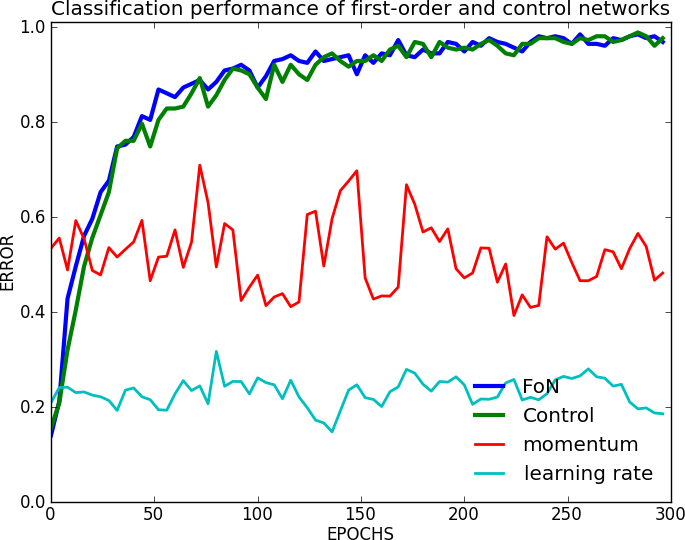
\includegraphics[width=250px]{data/expD4/perf.png}
	  &
	  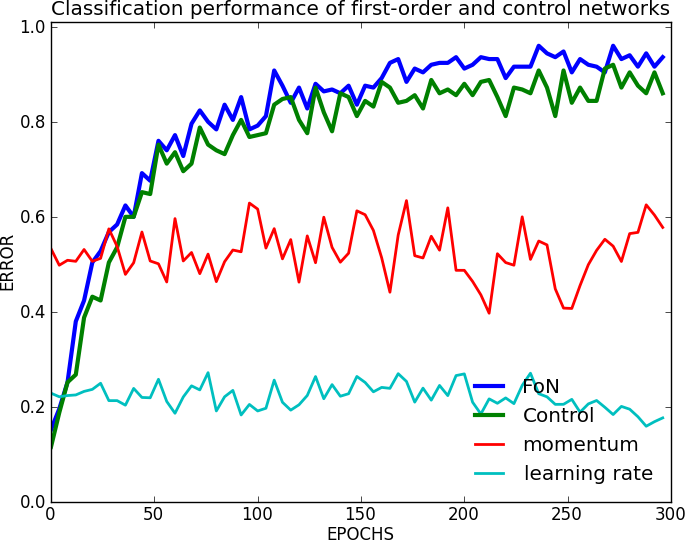
\includegraphics[width=250px]{data/expD4/perf_100.png} 
	\end{tabular}
      \end{center} 
      \subparagraph{Notes}
	\begin{itemize}
	  \item la performance de classification représente le taux de bonnes réponses (winner-take-all) pour les 50 formes présentées sur une époque
	  \item momentum et learning rate sont la moyenne des paramètres appliquées au premier réseau sur une époque
	\end{itemize}
      \subparagraph{Conclusion}
	\begin{itemize}
	  \item il y a une légère hausse de performance par rapport à un réseau de base, elle est plus accentuée lorsque le nombre de neurones dans
	  la couche cachée est élevé
	\end{itemize}
    \paragraph{Secondaires}
       Analyse des performances RMS
      \begin{center}
	\begin{tabular}{lr}
	  \hspace*{-1cm}
	  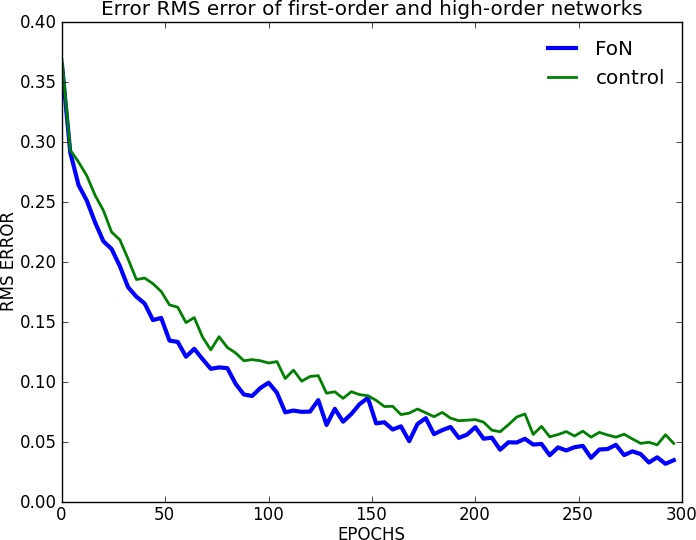
\includegraphics[width=250px]{data/expD4/rms.png}
	  &
	  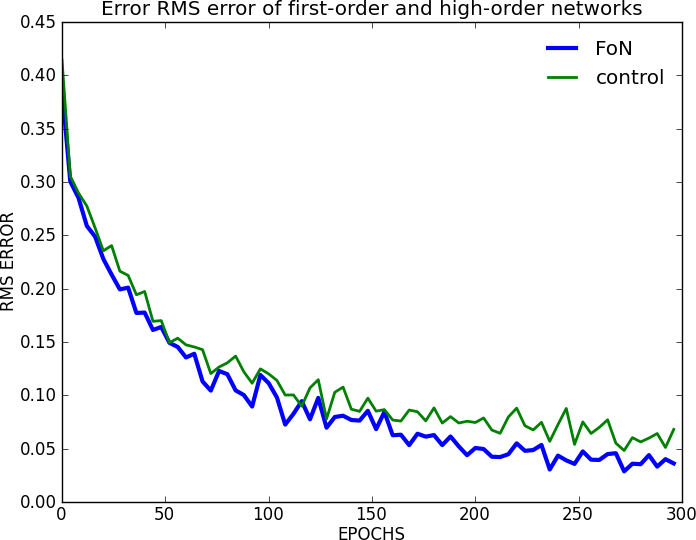
\includegraphics[width=250px]{data/expD4/rms_100.png} 
	\end{tabular}
      \end{center} 
      \subparagraph{Notes}
	\begin{itemize}
	  \item formule utilisée pour RMS (cf. Formules~\nameref{rms})
	\end{itemize}
      \subparagraph{Conclusion}
	Le RMS ne nous dit pas grand chose de plus que la performance de classification.

  \subsection{Conclusion}
  L'expérience est plutôt concluente, mais le système d'encodage/décodage du perceptron à apprentissage par renforcement 
  peut probablement être amélioré.
  

  \newpage 
  \subsection{Formules}
    \paragraph{RMS} \label{rms}
  Pour une époque $e$ :
  \begin{center}
    \begin{large}
    $ rms_{e} = \sqrt{ \frac{1}{n} \sum \limits_{i=1}^{n} 
    ( o_{i,e} - d_{i} )^2 } $
    \end{large}
  $ with \left\lbrace \begin{array}{lll} n : number\ of\ neurons\ on\ the\ output\ 
  layer\\o_{i,e} : value\ obtained\ for\ the\ i^{th}\ neuron\ at\ the\ e^{th}\ epoch\\d_{i} : 
  value\ desired \ for\ the\ i^{th}\ neuron\end{array} \right.$
  \end{center}
    
    \paragraph{Descente de gradient} \cite{Touzet_1992} \\
  Construction de l'erreur : 
    \begin{center}
      $y_{i} = f'(a_i) \times ( d_i - x_i ) \ si\ i\ neurone\ de\ sortie $ \\
      $y_{i} = f'(a_i) \times \sum \limits_{k} ( w_{ki} \times y_k )\ si\ i\ neurone\ cache $
    \end{center}
  Mise à jour des poids :
    \begin{center}
      $w_{ij}(t+1) = w_{ij}(t) + learning\_rate \times y_{i} \times x_j + momentum \times 
      (w_{ij}(t) - w_{ij}(t-1) )$
    \end{center}
  Variables : 
    \begin{center}
      $\left\lbrace \begin{array}{lll} 
	f : fonction\ sigmoide \\
	x_i : valeur\ du\ neurone\ i\\
	d_i : valeur\ desire pour\ le\ neurone\ i\\
	a_i : somme\ pondere\ des\ poids\ du\ neurone\ i
      \end{array} \right.$
    \end{center}
    
\bibliographystyle{../pre-rapport/apalike}
\bibliography{../pre-rapport/biblio}
